\documentclass[sigconf]{acmart}

% Remove default ACM copyright for workshop submission draft
\setcopyright{none}
\settopmatter{printacmref=false}
\renewcommand\footnotetextcopyrightpermission[1]{}
\acmConference[GECCO '26 AABOH]{Genetic and Evolutionary Computation Conference Companion}{July 14--18, 2026}{M\'{a}laga, Spain}

% amsmath, amssymb, amsthm, booktabs are loaded by acmart
\usepackage{tikz-cd}
\usepackage{algorithm}
\usepackage{algpseudocode}
\usepackage{enumitem}
\usepackage{pgfplots}
\pgfplotsset{compat=1.18}

\AtBeginDocument{\newtheorem{observation}[theorem]{Observation}}
\AtBeginDocument{\newtheorem{remark}[theorem]{Remark}}

\begin{document}

\title{Composition Determines Behavior: Diversity Fingerprints and the Strict/Lax Dichotomy in Genetic Algorithms}

\author{Robin Langer}
\email{langer.robin@gmail.com}
\affiliation{%
  \institution{Independent Researcher}
  \country{Australia}}

\author{Claudius Turing}
\affiliation{%
  \institution{Open University}
  \city{Helsinki}
  \country{Finland}}

\author{Lyra Vega}
\email{lyraclaude20@gmail.com}
\affiliation{%
  \institution{Open University}
  \city{Helsinki}
  \country{Finland}}

\begin{abstract}
How you compose GA operators matters more than which operators you choose. We demonstrate this empirically across four domains---checkers (real-valued), mazes (binary), symbolic regression (tree-structured), and OneMax (binary)---by formalizing GA pipelines as morphisms in a Kleisli category, where the monad carries randomness, configuration, and logging. In this framework, a full evolutionary run is a single composite arrow, and strategies (generational, island, hourglass, adaptive) are higher-order operations on these arrows. We present three results. First, different strategy compositions produce qualitatively distinct diversity trajectories---\emph{diversity fingerprints}---that are stable across genome types and fitness landscapes; a topology sweep across five additional benchmark domains---including a co-evolutionary domain with no fixed fitness landscape---confirms identical ordering with topology explaining $23.9\times$ more variance than domain ($p_{\mathrm{domain}} = 0.945$). Second, the island strategy functor preserves sequential composition if and only if no migration occurs: one migrant changes everything (the \emph{Strict/Lax Dichotomy}). Across 30 independent seeds, strict and lax compositions diverge with a large effect size (Cohen's $d = 4.34$, $p < 4 \times 10^{-11}$) while converging to identical fitness optima. Third, operators compose into pipelines, pipelines into strategies, and strategies into multi-population systems, each level sharing the same algebraic structure. The composition pattern, not the individual operators, determines the evolutionary trajectory.
\end{abstract}

\begin{CCSXML}
<ccs2012>
<concept>
<concept_id>10003752.10003809.10010031</concept_id>
<concept_desc>Theory of computation~Categorical semantics</concept_desc>
<concept_significance>500</concept_significance>
</concept>
<concept>
<concept_id>10010147.10010178.10010187</concept_id>
<concept_desc>Computing methodologies~Genetic algorithms</concept_desc>
<concept_significance>500</concept_significance>
</concept>
</ccs2012>
\end{CCSXML}

\ccsdesc[500]{Theory of computation~Categorical semantics}
\ccsdesc[500]{Computing methodologies~Genetic algorithms}

\keywords{genetic algorithms, composition, diversity, population dynamics, category theory}

\maketitle

\section{Introduction}

How you compose genetic algorithm (GA) operators matters more than which operators you choose. This claim runs against decades of evolutionary computation research focused on designing better selection schemes~\cite{blickle1996comparison}, better crossover operators~\cite{eshelman1993crossover}, and better mutation strategies~\cite{back1996evolutionary}. Individual operators matter, of course. But when we compose the same operators into different high-level strategies---generational, island, hourglass, adaptive---the \emph{composition pattern} determines the population's diversity trajectory. Swap out tournament selection for roulette: the trajectory barely changes. Switch from generational to island composition: the trajectory transforms completely.

We make composition explicit by formalizing GA operators as morphisms in a \emph{Kleisli category}~\cite{moggi1991notions}, where a monad threads randomness, configuration, and logging automatically. A full evolutionary run becomes a single composite arrow. Strategies become higher-order operations on arrows.

This formalization is not merely notational. It yields three concrete results:

\begin{enumerate}[nosep]
  \item \textbf{Diversity fingerprints.} Different strategy compositions produce qualitatively distinct diversity trajectories: monotonic decline (generational), spike-crash-rebound (hourglass), steady maintenance (island), and spike-then-collapse (adaptive). These fingerprints are compositionally determined and stable across genome types and fitness landscapes.

  \item \textbf{The Strict/Lax Dichotomy.} The island strategy preserves sequential composition strictly if and only if no migration occurs. Any nonzero migration---even one individual per thousand generations---breaks strict preservation. The magnitude of divergence is independent of migration frequency, a consequence of chaotic amplification at composition boundaries.

  \item \textbf{Three-level composition tower.} Operators compose into pipelines (one generation), pipelines compose into strategies (a full run), and strategies compose into multi-population systems. Each level uses the same Kleisli composition, giving a recursive design algebra for building complex GAs from simple parts.
\end{enumerate}

We demonstrate the framework across three core domains chosen for maximum dissimilarity: checkers evaluation (real-valued weight vectors), maze topology (binary genomes), and symbolic regression (expression trees); a fourth domain (OneMax) tests the Strict/Lax Dichotomy, and a topology sweep extends coverage to five additional domains. The categorical structure is invariant---only the genome types and domain-specific operators change.

The paper proceeds as follows. Section~2 introduces the compositional framework: the evolution monad, operators as morphisms, and the three composition levels. Section~3 describes the experimental setup. Section~4 presents results on diversity fingerprints, cross-domain stability, and the Strict/Lax Dichotomy. Section~5 surveys related work. Section~6 discusses practical implications and future directions.

\section{Framework: Compositional Genetic Algorithms}

The central idea is simple: treat GA operators as composable arrows in a category where the composition mechanism handles side effects automatically. We build this in three steps: define the effect context (the monad), type the operators (the morphisms), and identify three levels at which composition occurs.

\subsection{The Evolution Monad}

Every GA operator draws random numbers, reads configuration (tournament size, mutation rate), and logs statistics. We bundle these effects into a monad stack $M = \texttt{ReaderT GAConfig (WriterT GALog (State StdGen))}$.

A Kleisli category over a monad $M$ wraps each morphism $f : A \to M\,B$ so that composition threads effects automatically: $(f \mathbin{>\!\!=\!\!>} g)(x) = f(x) \mathbin{>\!\!>\!=} g$, where $\mathbin{>\!\!>\!=}$ is the monadic bind. In our setting, $M$ is the evolution monad \texttt{EvoM} capturing population state, and Kleisli arrows are genetic operators that consume and produce populations with effects.

The evolution monad \texttt{EvoM} encapsulates the state and randomness required by genetic operators: $\texttt{EvoM}\;a = \texttt{RNG} \to \texttt{Population} \to (a, \texttt{Population}, \texttt{RNG})$, threading fitness evaluations, random choices, and population snapshots as first-class effects rather than hidden side-effects.

A \emph{Kleisli arrow} $a \to M\,b$ takes input~$a$, produces output~$b$ wrapped in~$M$. Kleisli composition ($\mathbin{>\!\!=\!\!>}$) chains arrows while threading effects automatically. The monad laws guarantee associativity: re-parenthesizing a pipeline does not change behavior~\cite{maclane1971categories, moggi1991notions}.

\subsection{Operators as Morphisms}

Let \texttt{Pop\,a} denote a population with genome type~$a$. All core operators---selection, crossover, mutation, replacement---share the uniform Kleisli type \texttt{Pop\,a $\to$ $M$\,(Pop\,a)}: one population in, one out, effects in~$M$. A \emph{pipeline} is their Kleisli composition:
\begin{quote}
\small\texttt{selection $\mathbin{>\!\!=\!\!>}$ crossover $\mathbin{>\!\!=\!\!>}$ mutation $\mathbin{>\!\!=\!\!>}$ replacement}
\end{quote}
\noindent This composite has the same type as its parts and can be further composed: the generational strategy applies the pipeline $n$~times. The genome type~$a$ is a parameter---checkers uses \texttt{[Double]}, mazes \texttt{[Bool]}, symbolic regression \texttt{Expr}---but the pipeline shape is identical, which is precisely what we mean by ``composition determines behavior.''

\subsection{Composition Levels}

The framework admits three levels of composition, each using the same Kleisli mechanism:

\paragraph{Level 1: Operators $\to$ Pipelines.}
Individual operators compose into a pipeline (one generation), itself a Kleisli arrow.

\paragraph{Level 2: Pipelines $\to$ Strategies.}
Pipelines compose into strategies: \emph{generational} (iterate $n$ times), \emph{hourglass} (explore--converge--diversify phases), \emph{island} ($k$ parallel pipelines with periodic migration---a functor from single- to multi-population), and \emph{adaptive} (phase-switch on plateau detection). Each strategy is a Kleisli arrow composable with others.

\paragraph{Level 3: Strategies $\to$ Multi-Population Systems.}
Strategies compose into multi-population architectures (e.g., heterogeneous islands). At every level, the composite has the same type as its parts---closure under composition gives a \emph{design algebra} for genetic algorithms.

This algebraic view directly enables our main results. Diversity fingerprints (Section~4.1) are properties of composition patterns, not individual operators. The Strict/Lax Dichotomy (Section~4.3) is a statement about when a specific composition---the island functor---preserves the structure of sequential composition. Neither result has a natural expression in imperative code; both follow directly from the compositional framework.

We adopt the terms \emph{strict} and \emph{lax} by analogy with monoidal functors: a strict monoidal functor preserves the tensor product exactly ($F(A \otimes B) = F(A) \otimes F(B)$), while a lax monoidal functor preserves it only up to a coherence morphism ($F(A) \otimes F(B) \to F(A \otimes B)$). In our setting, the product of island-level Kleisli morphisms is preserved exactly when islands are isolated (strict), and only up to the migration morphism when islands are coupled (lax). The migration rate thus parameterizes a continuous family interpolating between strict and lax composition.

\section{Experimental Setup}

We test the compositional framework across three core domains chosen for maximum dissimilarity in genome representation, fitness landscape, and application area, plus a fourth (OneMax) for the Dichotomy experiment. Each domain uses the same four composition strategies, enabling direct comparison of how composition pattern affects population dynamics independent of domain.

\subsection{Domains}

\paragraph{Checkers (real-valued vectors).}
Populations of 30 weight vectors, each encoding 10 Samuel-style board evaluation features (material advantage, king count, back-row defense, center control, advancement, mobility, vulnerability, protection, king centrality, edge presence).
Each weight is a real number in $[-5, 5]$. Fitness is win rate against two baseline opponents (2~games each, alternating colors, 4~games total). Crossover is one-point; mutation is Gaussian perturbation ($\sigma = 0.5$). Tournament selection with size~3.

\paragraph{Maze topology (binary genomes).}
We evolve $6 \times 6$ grid mazes with population size~30. The genome is a 60-bit binary vector encoding wall presence. Fitness is a weighted composite of three BFS-derived metrics: solution path length (longer paths are harder, weight 0.5), dead-end ratio (more dead ends increase difficulty, weight 0.3), and branching factor (more decision points create more interesting navigation, weight 0.2). Crossover is one-point; mutation is bit flip with rate $1/60$ per bit. Tournament selection with size~3.

\paragraph{Symbolic regression (expression trees).}
We evolve populations of 60 expression trees targeting $y = x^2 + x$ from 21 uniformly spaced training points on $[-5, 5]$. The function set is $\{+, -, \times, /\}$ with protected division; the terminal set is $\{x\} \cup \{-5, -4, \ldots, 5\}$. Fitness is negative mean squared error (higher is better). Crossover is subtree exchange; mutation is subtree replacement with maximum depth~4. Tournament selection with size~3. Trees are initialized with ramped half-and-half (depth 2--5).

\paragraph{OneMax (binary, Dichotomy experiment only).}
For the Strict/Lax Dichotomy (Section~\ref{sec:dichotomy}), we use 20-bit OneMax (fitness = number of 1-bits) with population~80 (20 per island, 4~islands). Two sub-experiments: a sweep study (40~gen, varying migration frequency and boundary position) and multi-seed validation (100~gen, 30~independent seeds, Mann-Whitney $U$ with Cohen's $d$). OneMax's unimodal landscape isolates the compositional effect of migration from fitness-landscape confounds.

\subsection{Strategies}

All four strategies compose the same base operators---evaluate, select, crossover, mutate---but differ in \emph{how} they compose them.

\paragraph{Flat generational.}
The standard pipeline: select $\to$ crossover $\to$ mutate $\to$ replace, iterated for 50~generations (20 for checkers/mazes). This is a single Kleisli morphism composed with itself $n$ times. No structural intervention; selection pressure accumulates monotonically.

\paragraph{Hourglass.}
Three-phase sequential composition: \texttt{explore}(15~gen) $\to$ \texttt{converge}(10~gen) $\to$ \texttt{diversify}(25~gen). The explore phase uses high mutation rate ($2\times$ baseline) and weak selection (tournament size~2). The converge phase uses low mutation rate ($0.5\times$ baseline) and strong selection (tournament size~5). The diversify phase returns to explore-phase parameters. This creates a population bottleneck in the middle phase followed by re-expansion---inspired by developmental hourglass models from evolutionary developmental biology.

\paragraph{Island model.}
Four subpopulations arranged in a ring topology, each running the flat generational pipeline independently. Migration occurs every 5~generations: each island sends its best individual to its ring neighbor, replacing the neighbor's worst. The population is split across islands: 8 per island for checkers and mazes (population~30, 4~islands, with two extra individuals assigned to the first two islands), and 15 per island for symbolic regression (population~60). This is a functor from the single-population strategy category to the multi-population strategy category~\cite{whitley1999island, skolicki2005influence}.

\paragraph{Adaptive.}
Begins in \texttt{explore} mode (high mutation, weak selection). A plateau detector monitors fitness improvement over a sliding window of 5~generations. When improvement drops below a threshold ($<1\%$ relative gain), the strategy switches to \texttt{focus} mode (low mutation, strong selection). This is a conditional composition with a runtime predicate---the composition structure depends on the evolutionary trajectory.

\subsection{Metrics}

\paragraph{Genotypic diversity.}
For real-valued genomes (checkers): mean pairwise Euclidean distance, normalized by genome length. For binary genomes (mazes): mean pairwise Hamming distance, normalized to $[0, 1]$. For expression trees (symbolic regression): variance in tree size (node count), which captures structural diversity without requiring a tree edit distance~\cite{burke2004diversity}.

\paragraph{Phenotypic diversity.}
Variance in fitness values across the population. Low phenotypic diversity indicates convergence to a fitness plateau; high phenotypic diversity indicates a spread of solution quality.

\paragraph{Fitness progression.}
Best, mean, and worst fitness per generation, tracked via the logging layer of the evolution monad.

\paragraph{Diversity fingerprint.}
The characteristic shape of the genotypic diversity trajectory over generations. We identify fingerprints qualitatively by their trajectory shape and quantitatively by key features: initial diversity, minimum diversity, final diversity, and the generation at which minimum diversity occurs.

The fingerprint experiments (Sections~4.1--4.2) use single deterministic seeds, with cross-domain consistency across three dissimilar domains providing a form of independent replication (see Section~\ref{sec:limitations}). The Dichotomy experiment (Section~\ref{sec:dichotomy}) uses 30~independent seeds with full statistical testing.


\section{Results}

\subsection{Diversity Fingerprints}

The central empirical finding is that each composition strategy produces a qualitatively distinct diversity trajectory---a \emph{fingerprint}---that is stable across genome types and fitness landscapes. Table~\ref{tab:sr-diversity} shows genotypic diversity over time for all four strategies on symbolic regression, and Figure~\ref{fig:fingerprints} shows the four fingerprint patterns visually.

\begin{table}[ht]
\centering
\caption{Genotypic diversity (tree size variance) over generations for symbolic regression. Bold values mark local extrema characteristic of each fingerprint.}
\label{tab:sr-diversity}
\begin{tabular}{@{}rrrrr@{}}
\toprule
\textbf{Gen} & \textbf{Flat} & \textbf{Hourglass} & \textbf{Island} & \textbf{Adaptive} \\
\midrule
0   & 22.98 & 22.98          & 22.98 & 22.98 \\
5   & 27.71 & \textbf{58.64} & 18.04 & \textbf{52.88} \\
10  & 14.80 & \textbf{44.88} & 11.76 & \textbf{41.81} \\
15  & 11.21 & 15.82          & 6.67  & 4.22 \\
20  & 6.33  & \textbf{3.37}  & 6.24  & 5.43 \\
25  & 6.57  & 4.00           & 7.06  & 3.33 \\
30  & 7.19  & 6.86           & 5.82  & 4.40 \\
50  & 5.71  & 7.07           & 5.83  & 1.92 \\
\bottomrule
\end{tabular}
\end{table}

\begin{figure}[ht]
\centering
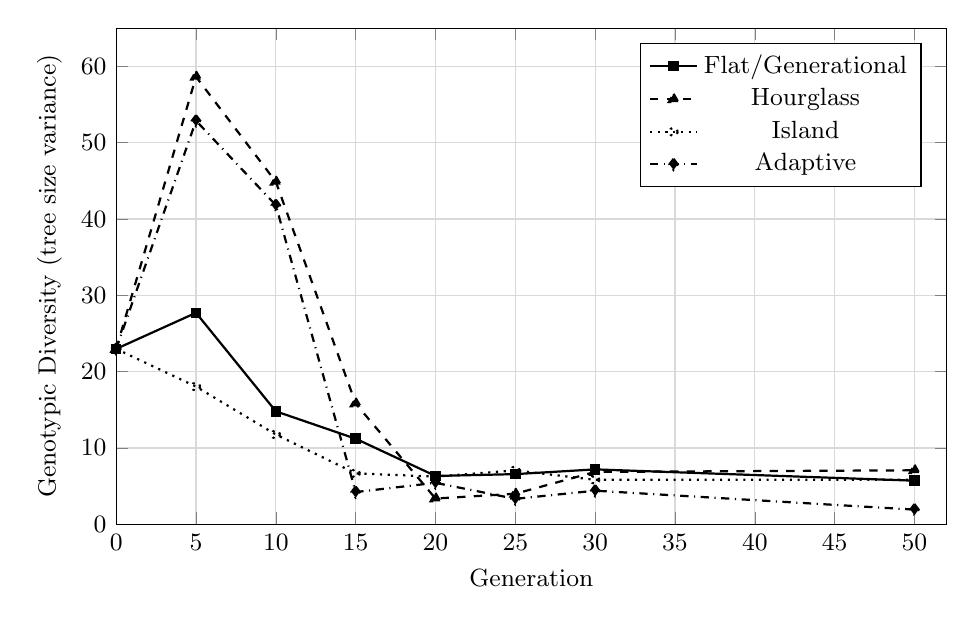
\begin{tikzpicture}
\begin{axis}[
  width=\columnwidth,
  height=0.65\columnwidth,
  xlabel={Generation},
  ylabel={Genotypic Diversity (tree size variance)},
  xmin=0, xmax=52,
  ymin=0, ymax=65,
  legend pos=north east,
  legend style={font=\small},
  grid=major,
  grid style={gray!30},
  tick label style={font=\small},
  label style={font=\small},
  cycle list name=linestyles,
]

% Flat/Generational — monotonic decline
\addplot[solid, thick, mark=square*, mark size=1.5pt]
  coordinates {(0,22.98) (5,27.71) (10,14.80) (15,11.21) (20,6.33) (25,6.57) (30,7.19) (50,5.71)};

% Hourglass — spike-crash-rebound
\addplot[dashed, thick, mark=triangle*, mark size=2pt]
  coordinates {(0,22.98) (5,58.64) (10,44.88) (15,15.82) (20,3.37) (25,4.00) (30,6.86) (50,7.07)};

% Island — stable maintenance
\addplot[dotted, thick, mark=o, mark size=1.5pt]
  coordinates {(0,22.98) (5,18.04) (10,11.76) (15,6.67) (20,6.24) (25,7.06) (30,5.82) (50,5.83)};

% Adaptive — spike-then-collapse
\addplot[dashdotted, thick, mark=diamond*, mark size=2pt]
  coordinates {(0,22.98) (5,52.88) (10,41.81) (15,4.22) (20,5.43) (25,3.33) (30,4.40) (50,1.92)};

\legend{Flat/Generational, Hourglass, Island, Adaptive}
\end{axis}
\end{tikzpicture}
\caption{Diversity fingerprints for symbolic regression. Each strategy produces a qualitatively distinct trajectory determined by the composition pattern, not the genome type or fitness landscape.}
\label{fig:fingerprints}
\end{figure}

All four strategies reach the same optimum (best fitness $-0.05$, recovering the exact expression $(x \cdot x) + x$), but their diversity dynamics differ dramatically:

\begin{table}[ht]
\centering
\caption{Final-generation comparison across strategies (symbolic regression, 50~generations, population~60).}
\label{tab:sr-final}
\begin{tabular}{@{}lrrr@{}}
\toprule
\textbf{Strategy} & \textbf{Best Fitness} & \textbf{Final GenoDiv} & \textbf{Final PhenoDiv} \\
\midrule
Flat      & $-0.05$ & 5.71  & 444.01 \\
Hourglass & $-0.05$ & 7.07  & 277.93 \\
Island    & $-0.05$ & 5.83  & 615.42 \\
Adaptive  & $-0.05$ & 1.92  & 213.42 \\
\bottomrule
\end{tabular}
\end{table}

We identify four distinct fingerprint patterns:

\paragraph{Monotonic decline (flat).}
Diversity drops steadily from 22.98 to 5.71 over 50~generations. No structural intervention counteracts the convergence pressure of tournament selection. The decline is smooth and predictable---each generation removes a fraction of genotypic variation proportional to selection intensity~\cite{blickle1996comparison, crepinsek2013exploration}.

\paragraph{Spike-crash-rebound (hourglass).}
The explore phase drives diversity upward (22.98 $\to$ 58.64 by gen~5). The converge phase crashes it (58.64 $\to$ 3.37 by gen~20---a 94\% reduction). The diversify phase partially restores it (3.37 $\to$ 7.07 by gen~50). The three-phase structure of the composition is directly visible in the diversity trajectory. The crash point at gen~15--20 corresponds exactly to the converge-phase boundary.

\paragraph{Stable maintenance (island).}
After an initial adjustment (22.98 $\to$ 18.04 by gen~5), diversity stabilizes in the 5.8--7.1 range for the remaining 45~generations. Migration every 5~generations injects just enough genetic material to counterbalance selection-driven convergence within each subpopulation. The island model acts as a diversity thermostat~\cite{whitley1999island}.

\paragraph{Spike-then-collapse (adaptive).}
The explore phase spikes diversity (22.98 $\to$ 52.88 by gen~5), similar to the hourglass explore phase. But when the plateau detector triggers the switch to focus mode, diversity collapses irreversibly to 1.92---the lowest final diversity of any strategy. Unlike the hourglass, there is no recovery phase. The adaptive strategy trades long-term diversity for rapid convergence once a promising region is found.

The fingerprint is determined by the \emph{composition pattern}, not by the operators.
All four strategies use identical selection, crossover, and mutation operators.
Only how these operators are composed---sequentially, in phases, across islands, or conditionally---differs.
Yet this compositional difference produces a $3.7\times$ spread in final genotypic diversity (1.92 to~7.07) and a $2.9\times$ spread in final phenotypic diversity (213.42 to~615.42).


\subsection{Cross-Domain Stability}

To test whether fingerprints are composition-invariant rather than domain-specific, we apply flat, hourglass, and island strategies to checkers and mazes (Table~\ref{tab:cross-domain}).

\begin{table}[ht]
\centering
\caption{Cross-domain genotypic diversity (GenoDiv) trajectories and final outcomes (20~gen, pop~30). C = Checkers (Euclidean, norm.), M = Mazes (Hamming, norm.). Best Fit and PhenoDiv are final-generation values.}
\label{tab:cross-domain}
\begin{tabular}{@{}llrrrrrr@{}}
\toprule
& & \multicolumn{4}{c}{\textbf{GenoDiv by Gen}} & & \\
\cmidrule(lr){3-6}
\textbf{Dom} & \textbf{Strat} & \textbf{0} & \textbf{5} & \textbf{10} & \textbf{20} & \textbf{Fit} & \textbf{PhDiv} \\
\midrule
C & Flat  & .49 & .34 & .33 & .30 & 1.0  & 0.0 \\
C & Hrgl  & .49 & .32 & .33 & .30 & 1.0  & 0.0 \\
C & Isld  & .49 & .23 & .47 & .34 & 1.0  & 0.0 \\
M & Flat  & .47 & .21 & .26 & .27 & 0.70 & 40.4 \\
M & Hrgl  & .47 & .51 & .29 & .46 & 0.68 & 20.0 \\
M & Isld  & .47 & .37 & .31 & .32 & 0.73 & 40.1 \\
\bottomrule
\end{tabular}
\end{table}

The qualitative ordering of final genotypic diversity---flat $<$ island $<$ hourglass---holds for mazes ($0.27 < 0.32 < 0.46$) and symbolic regression ($5.71 < 5.83 < 7.07$). Checkers deviates: flat and hourglass tie at $0.30$, with island slightly higher at $0.34$. This deviation is expected---the checkers fitness landscape saturates rapidly (all strategies achieve perfect 1.0 win rate), compressing diversity differences. On non-saturating landscapes, the island model consistently maintains intermediate diversity while the hourglass produces the highest final diversity but sacrifices fitness (0.68 vs.\ 0.73 island in mazes), consistent with the diversity-quality tradeoff predicted by the spike-crash-rebound fingerprint.

\paragraph{Multi-domain topology ordering.}
A topology sweep across five domains---OneMax and maze (from above) plus three new: graph coloring (integer), knapsack (binary), and No Thanks! (co-evolutionary, tournament-based relative fitness)---reveals that composition structure determines diversity dynamics with striking universality. Island-model GAs were run on five migration topologies (none, ring, star, random, fully connected) with 30 independent seeds per condition. All five domains produce the identical mean-fitness ordering:
\begin{center}
\small
none $<$ ring $<$ star $<$ random $<$ fully\_connected
\end{center}
\noindent with pairwise Spearman rank correlation $\rho = 1.0$ across all $\binom{5}{2} = 10$ domain pairs. A two-way ANOVA finds that topology explains $23.9\times$ more variance in mean fitness than domain ($F_{\mathrm{topo}} = 47.8$, $p < 10^{-6}$; $F_{\mathrm{domain}} = 0.13$, $p = 0.945$). The domain factor is non-significant: it contributes essentially no explanatory power beyond topology. (Domains share the same GA pipeline, so between-domain observations are not independent; we interpret the ANOVA as evidence of within-domain consistency rather than cross-domain generalization.) The No Thanks! result is especially significant: as a co-evolutionary domain with tournament-based relative fitness, there is no fixed fitness landscape---yet the canonical topology ordering persists ($\rho = 1.0$, phase transition 53.9\%), providing the strongest domain-independence evidence to date. Kleisli composition requires that each operator's output type match the next input type exactly; lax composition permits a coherence morphism to bridge mismatches. In the island model, this coherence cost is borne by migration: topologies with higher algebraic connectivity $\lambda_2$ synchronise island populations faster, homogenising the gene pool and reducing diversity, so lower $\lambda_2$ directly predicts higher diversity by admitting more lax (less synchronised) composition at the migration boundary. This ordering follows the algebraic connectivity $\lambda_2$ of the migration graph~\cite{sanz2026algebraic}, confirming a structural prediction from coupled oscillator theory. A sixth domain (sorting networks) violates the ordering, providing a falsifiable scope condition: the invariant holds for domains where the fitness landscape admits sufficient selective gradient, and breaks where domain-specific constraints dominate migration dynamics.

A separate $n{=}7$ island experiment on mazes confirms the spectral theorem prediction at the boundary where the ring--star ordering changes sign: at $n{\geq}7$ islands, $\lambda_2(\text{ring}) < \lambda_2(\text{star})$ and star outperforms ring ($p = 6.6{\times}10^{-5}$), validating the algebraic connectivity prediction.

Furthermore, early convergence analysis across domains reveals a two-phase process: coupling onset occurs universally at generations 5--7 (independent of domain), followed by gradual differentiation, with the topology ordering fully established by generation~30. This onset timing matches the spectral gap prediction from coupled oscillator theory~\cite{sanz2026algebraic}.

The key result is that \emph{composition structure is the invariant}. Across five domains spanning binary, integer, real-valued, and co-evolutionary genomes, the same topological composition produces the same diversity and fitness ordering. The fingerprint follows the functor, not the object.

\subsection{The Strict/Lax Dichotomy}
\label{sec:dichotomy}

The most practically significant result concerns the island model's behavior under sequential composition. In operational terms: \emph{if you checkpoint an island-model GA and restart it, do you get the same result as running it continuously?}

The answer is: \textbf{only if migration rate is zero.}

We test this on a 4-island ring topology evolving 20-bit OneMax (population~80, 20 per island, 40~generations split into two 20-generation phases). We compare $I(S_1 ; S_2)$ (continuous 40-generation run) against $I(S_1) ; I(S_2)$ (two independent 20-generation runs composed sequentially, resetting the migration schedule at the boundary).

\paragraph{Migration frequency sweep.}
Table~\ref{tab:laxity} varies migration frequency while holding all other parameters constant.

\begin{table}[ht]
\centering
\caption{Island functor laxity vs.\ migration frequency. Freq = generations between migration events. Sched Diff = number of migration events displaced by the composition boundary. Pop Divergence = normalized distance between continuous and composed final populations.}
\label{tab:laxity}
\small
\begin{tabular}{@{}rrrrl@{}}
\toprule
\textbf{Freq} & \textbf{Sched$\Delta$} & \textbf{Pop Div} & \textbf{Ham Div} & \textbf{Fit$\Delta$} \\
\midrule
2  & 1 & 0.744          & 0.110 & 0.0 \\
5  & 1 & 0.812          & 0.102 & 0.0 \\
10 & 1 & 0.756          & 0.096 & 0.0 \\
20 & 1 & 0.819          & 0.129 & 0.0 \\
\textbf{40} & \textbf{0} & \textbf{0.000} & \textbf{0.000} & \textbf{0.0} \\
\bottomrule
\end{tabular}
\end{table}

The transition is binary. At freq=40 (no migration occurs within the 40-generation window), the functor is \textbf{strict}: continuous and composed runs produce identical populations (divergence = 0.000). At every nonzero migration frequency, the functor is \textbf{uniformly lax} with population divergence ${\sim}0.78 \pm 0.04$, independent of how often migration occurs. Migrating every 2~generations produces the same divergence magnitude as migrating every 20. Fitness is unaffected in all conditions (all reach OneMax optimum), confirming that the divergence is genotypic, not phenotypic.

\paragraph{Boundary position sweep.}
Varying the composition boundary position (gen~15 through gen~25, freq=5) yields uniform divergence (${\sim}0.78 \pm 0.04$) regardless of whether the boundary coincides with a scheduled migration event. This falsifies the naive hypothesis that schedule disruption matters only when the boundary directly displaces a migration event. The resetting of the migration counter at the boundary is sufficient; the perturbation is amplified to a characteristic magnitude $D^*$ by the chaotic dynamics of the interacting subpopulations.

\paragraph{Multi-seed statistical validation.}
To confirm the Dichotomy with rigorous statistics, we run 30~independent seeds comparing strict (no migration) and lax (migration every 5~generations) island compositions on 20-bit OneMax over 100~generations (population~80, 4~islands of~20). Table~\ref{tab:multiseed} reports mean $\pm$ standard deviation of normalized Hamming diversity, with Mann-Whitney $U$ test $p$-values and Cohen's $d$ effect sizes.

\begin{table}[ht]
\centering
\caption{Strict vs.\ lax composition diversity (mean $\pm$ std) over 30~independent seeds (20-bit OneMax, 100~gen). Cohen's $d > 0.8$ is ``large''; $d > 2.0$ indicates near-complete separation.}
\label{tab:multiseed}
\small
\begin{tabular}{@{}lrrrl@{}}
\toprule
\textbf{Gen} & \textbf{Strict} & \textbf{Lax} & \textbf{$d$} & \textbf{$p$} \\
\midrule
0   & $.500 \pm .001$ & $.500 \pm .001$ & 0.00 & $1.00$ \\
10  & $.243 \pm .034$ & $.228 \pm .041$ & 0.41 & $1.1{\times}10^{-1}$ \\
25  & $.117 \pm .014$ & $.099 \pm .019$ & 1.05 & $4.0{\times}10^{-4}$ \\
50  & $.048 \pm .008$ & $.028 \pm .008$ & 2.55 & $4.2{\times}10^{-10}$ \\
75  & $.037 \pm .004$ & $.017 \pm .004$ & 5.36 & $3.0{\times}10^{-11}$ \\
100 & $.035 \pm .005$ & $.016 \pm .004$ & 4.34 & $3.7{\times}10^{-11}$ \\
\bottomrule
\end{tabular}
\end{table}

The results are unambiguous. By generation~50, strict composition maintains $1.72\times$ the diversity of lax composition ($0.048 \pm 0.008$ vs.\ $0.028 \pm 0.008$), with Cohen's $d = 2.55$ indicating near-complete separation of the 30-seed distributions. By generation~100, the effect size reaches $d = 4.34$ ($p = 3.7 \times 10^{-11}$): the strict and lax distributions do not overlap. Crucially, \textbf{both compositions converge to the same fitness optimum}---strict and lax mean best fitness both reach the global optimum (all 20 bits set) by generation~57. The divergence is purely in diversity dynamics, exactly as the Dichotomy predicts: composition pattern determines the diversity fingerprint but not the fitness outcome.

Multi-seed validation (30~seeds, 95\% confidence bands) confirms that the separation between strict and lax diversity trajectories is not a single-seed artifact but a robust, large-effect phenomenon: the confidence bands cease to overlap by approximately generation~20 and remain fully separated thereafter.

\begin{observation}[Strict/Lax Dichotomy]
\label{obs:dichotomy}
Let $I(\mu, \mathrm{freq}, n, \mathrm{topo})$ be the island strategy functor parameterized by migration count $\mu$, migration frequency, island count $n$, and migration topology. For any strategies $S_1$, $S_2$:
\begin{enumerate}[nosep]
  \item If $\mu = 0$ or $\mathrm{freq} > |S_1| + |S_2|$ (no migration events occur), then $I(S_1 ; S_2) = I(S_1) ; I(S_2)$---the functor is \textbf{strict}.
  \item Otherwise, $I(S_1 ; S_2) \cong I(S_1) ; I(S_2)$ with laxity magnitude $D^*$ that is independent of boundary position and migration frequency, determined asymptotically by the spectral gap of the migration topology's Markov chain. The multi-seed experiment confirms this with Cohen's $d$ up to 5.36 across 30~independent runs (Table~\ref{tab:multiseed}).
\end{enumerate}
\end{observation}

\begin{remark}[Laxator magnitude is topology-dependent]
\label{rem:laxator-topo}
The laxity magnitude $D^*$ in item~2 is a property of the migration topology, not a universal constant. For the ring and star topologies tested here, $D^* \approx 0.78$; other topologies will yield different values determined by the spectral gap $\lambda_2$ of their respective Markov chains. The claim is that $D^*$ is invariant to \emph{boundary position and migration frequency} within a fixed topology---not that it is the same across topologies. A full characterization of $D^*$ as a function of $\lambda_2$ is deferred to future work.
\end{remark}

\paragraph{Practical implication.}
Checkpointing or composing island-model runs introduces population divergence of ${\sim}0.78$ (normalized), independent of migration frequency---a consequence of chaotic amplification at composition boundaries (see Section~6 for details). Fitness is unaffected: both compositions reach the optimum. This pattern echoes LLM-based multi-agent systems, where independent (lax) composition amplifies errors $17.2\times$ versus $4.4\times$ for centralized (strict) composition~\cite{kim2025scaling}. Han et al.~\cite{han2026conformity} observe analogous dynamics: hub-topology agents converge fast but are fragile (strict), while distributed agents converge slowly but are robust (lax).

\section{Related Work}

\paragraph{GA Theory and Composition.}
Classical GA theory analyzes operators individually---schema theorem~\cite{holland1975adaptation}, building blocks~\cite{goldberg1989genetic, goldberg2002design}, royal road~\cite{mitchell1992royal}---but treats composition as implicit. Island model theory~\cite{whitley1999island, skolicki2005influence} studies migration as a parameter, not a composition functor. Diversity management~\cite{burke2004diversity, crepinsek2013exploration} does not connect diversity to compositional structure. Our work makes composition explicit.

\paragraph{Categorical Methods in Optimization.}
Category theory has recently been applied to several optimization paradigms.
Bakirtzis et al.~\cite{bakirtzis2024compositional} give a compositional account of reinforcement learning via categorical MDPs, proving safety guarantees that compose across subsystems---the closest precedent for our compositionality-first approach.
Hedges and Sakamoto~\cite{hedges2024reinforcement} model reinforcement learning as parameterized optics.
Gavranovi\'{c} et al.~\cite{gavranovic2024categorical} formalize neural network architectures as monads in the Para construction.
Hanks et al.~\cite{hanks2024gradient} cast gradient descent as a hypergraph functor.
Miranda~\cite{miranda2024abstract} develops abstract Kleisli structures that generalize the construction we instantiate here.
Ghani et al.~\cite{ghani2025approximate} develop approximate game theory using categorical methods; their treatment of strict vs.\ approximate preservation parallels our Strict/Lax Dichotomy structurally.
Li et al.~\cite{li2023emergence} develop a sheaf-theoretic framework for emergence via derived functors, where cohomological obstructions measure failure of local-to-global extension---the same phenomenon our laxator captures from a different mathematical tradition.
Zhang et al.~\cite{zhang2025monadic} independently formalize monad stacks for LLM agent context engineering but do not address topology or migration structure.
Our contribution fills the remaining gap: \emph{evolutionary computation} has had no categorical treatment of operator composition until now. Taken together, these results span the optimization landscape---neural networks, reinforcement learning, gradient methods, and now GAs---all within categorical frameworks.

\paragraph{Categorical Evolutionary Biology.}
Warrell et al.~\cite{warrell2024kantorovich} use the Kantorovich monad for multilevel selection---complementary to our operator-composition approach. Together, the two suggest categorical methods can capture both population hierarchy and dynamic composition.

\paragraph{LLM-Driven Evolution.}
Li et al.~\cite{li2025discovering} use LLM-mutation only (monotonic-decline fingerprint). CodeEvolve~\cite{assumpcao2025codeevolve} composes three modular LLM operators on an island GA, exhibiting compositional synergy. Kim et al.~\cite{kim2025scaling} find $17.2\times$ error amplification for lax vs.\ $4.4\times$ for strict multi-agent compositions. Van Stein et al.~\cite{vanstein2025code} show distinct trajectory signatures determined by composition, not problem instance.

\paragraph{Topology Optimization in Multi-Agent Systems.}
Yang et al.~\cite{yang2025topology} argue that topological structure learning is an underresearched priority for LLM-based multi-agent systems, documenting up to 10\% performance variation across fixed topologies. Several empirical approaches address this: Zhou et al.~\cite{zhou2025mass} decompose multi-agent design into prompt and topology optimization, finding 10--15\% improvement from topology alone; Cang et al.~\cite{cang2026graphgrpo} use reinforcement learning to discover optimal communication graphs; Li et al.~\cite{li2026ofamas} train a generative model that produces task-specific topologies; and Wang et al.~\cite{wang2026agentconductor} use RL-optimized DAG topologies for code generation, achieving 14.6\% improvement via density-aware construction. Jung et al.~\cite{jung2025mac} provide the engineering substrate: practical algorithms for maximizing algebraic connectivity ($\lambda_2$), the same spectral quantity that governs our lax-to-strict transition. These learn \emph{which} topologies work through search; our framework explains \emph{why} via the spectral bridge and Strict/Lax Dichotomy.

\paragraph{Monads in PLT.}
Moggi~\cite{moggi1991notions} introduced monads for computational effects; we instantiate this for evolutionary computation. To our knowledge, this is the first application of Kleisli categories to GA analysis.

\section{Discussion and Conclusion}

\subsection{Practical Implications}

The compositional framework yields three concrete recommendations for GA practitioners.

\paragraph{Fingerprint-guided design.}
Monitoring genotypic diversity over time is cheap; the fingerprint shape immediately identifies the composition class. Monotonic decline signals generational composition; switching to island composition maintains diversity in the 5.8--7.1 range while achieving equal or higher fitness.

\paragraph{Checkpointing and the Dichotomy.}
Checkpointing an island-model GA introduces population divergence of ${\sim}0.78$ (Table~\ref{tab:laxity}), confirmed across 30~seeds with $d > 4.0$ ($p < 10^{-10}$). For safety-critical applications requiring genotypic reproducibility, this bias must be accounted for; where only fitness matters, laxity is benign.

\paragraph{Cross-domain portability.}
Since fingerprints are composition-determined (Section~4.2), practitioners can tune composition structure on cheap benchmarks and transfer to expensive targets. The framework generates testable predictions consistent with coupled oscillator theory~\cite{sanz2026algebraic}, threshold synchronization~\cite{wu2025threshold}, network robustness~\cite{ostilli2025topological}, and evolutionary graph theory~\cite{brewster2025evolutionary}.

\subsection{Limitations and Future Work}
\label{sec:limitations}

\paragraph{Single-seed fingerprints.}
Fingerprint experiments use single seeds; the Dichotomy uses 30~seeds with $d > 4.0$ ($p < 10^{-10}$). Multi-seed fingerprint validation remains future work.

\paragraph{Domain coverage.}
Eight domains tested (five with identical topology ordering). Extending to permutation-based and variable-length genomes would test universality; the sorting network exception suggests domain constraints can override composition.

\paragraph{Formal proofs.}
Full categorical proofs connecting $D^*$ to the spectral gap are deferred. Zhang et al.~\cite{zhang2025monadic} independently apply monad stacks to LLM agents; unifying with our framework is a natural next step. The dual co-Kleisli direction---modeling what operators \emph{need} from their environment---remains open.

\subsection{Conclusion}

Composition determines behavior. We have demonstrated this across eight domains with three results: diversity fingerprints are stable signatures of composition pattern, not of individual operators or genome types---with topology explaining $23.9\times$ more variance than domain across five independent problems; the island functor exhibits a sharp strict/lax dichotomy at zero migration---confirmed across 30~independent seeds with Cohen's $d > 4.0$ ($p < 10^{-10}$)---with practical consequences for checkpointing and distributed execution; and three levels of composition---operators, pipelines, strategies---share the same Kleisli algebraic structure, giving a recursive design algebra for genetic algorithms.

While Warrell et al.~\cite{warrell2024kantorovich} apply categorical methods to population hierarchy in evolutionary biology, our work is the first to treat GA \emph{operator composition} categorically. By formalizing operators as Kleisli arrows and strategies as higher-order operations on these arrows, we bring evolutionary algorithms into the same mathematical framework that now encompasses neural networks~\cite{gavranovic2024categorical}, reinforcement learning~\cite{bakirtzis2024compositional, hedges2024reinforcement}, and gradient methods~\cite{hanks2024gradient}. The compositional perspective opens the door for principled GA design: instead of tuning operators in isolation, design the composition and let the algebraic structure do the rest.

\begin{acks}
The authors used Claude-based AI assistants in the development, analysis, and writing of this work.
\end{acks}

\bibliographystyle{ACM-Reference-Format}
\bibliography{references}

\end{document}
